\documentclass[12pt,a4paper]{article}
\usepackage[utf8]{inputenc}
\usepackage[english]{babel}
\usepackage{float}
\usepackage{amsmath, amssymb}
\usepackage{graphicx}
\usepackage{tikz}
\usetikzlibrary{shapes.geometric, shapes.multipart, arrows.meta, positioning, calc, fit, backgrounds}
\usepackage{hyperref}
\usepackage{geometry}
\geometry{left=2.5cm, right=2.5cm, top=2.5cm, bottom=2.5cm}

\title{\textbf{Technical Report: Practical Byzantine Fault Tolerance (pBFT)}}
\author{Aldo Luna Bueno \\ 20170325B}
\date{\today}

\begin{document}

\maketitle
\tableofcontents
\newpage

\section{Foundations and Motivation}

\subsection{From ``Fail-Stop'' to ``Byzantine Fault''}
In the 1980s, fault tolerance research was heavily concentrated on \textit{fail-stop} faults, which occur when a node simply ceases to operate, typically due to a hardware crash. However, as systems grew more complex, these failures became just the tip of the iceberg. 

A node can fail due to software bugs or be compromised by malicious attackers. In these scenarios, the defective node does not shut down; it continues to communicate but can behave arbitrarily or transmit false information. This arbitrary behavior is known as a \textbf{Byzantine Fault}. Within a Byzantine environment, it is assumed that defective nodes actively conspire to corrupt the system state.

\subsection{The pBFT System Model}
The pBFT algorithm assumes a realistic and hostile system model:
\begin{itemize}
    \item \textbf{Asynchrony:} It operates in an asynchronous distributed system, such as the Internet, where messages can be delayed, lost, or delivered out of order.
    \item \textbf{Strong Adversary:} It posits an adversary capable of coordinating compromised nodes. pBFT relies heavily on cryptography (public-key signatures, MACs, cryptographic digests) to secure message integrity.
    \item \textbf{Safety without Synchrony:} It guarantees its safety property (contradictory operations will never be committed) regardless of network delays, relying only on weak synchrony for liveness.
\end{itemize}

\subsection{The $3f+1$ Rule}
To tolerate $f$ Byzantine failures, the minimum number of replicas required is $n = 3f+1$. This is because the protocol must be able to make progress using responses from $n - f$ replicas (since $f$ nodes could be dead or unresponsive). Within those received responses, $f$ nodes could be malicious liars. For the honest nodes' votes to strictly outvote the malicious ones, the following inequality must hold: $(n - f) - f > f \implies n > 3f$.

Another perspective to understand this rule is through quorum intersections. Committing an operation requires a quorum of $2f+1$ identical responses. If two distinct quorums of $2f+1$ intersect, their mathematical overlap will always contain at least $f+1$ replicas, inherently guaranteeing at least one honest node in the intersection.

\begin{figure}[H]
\centering
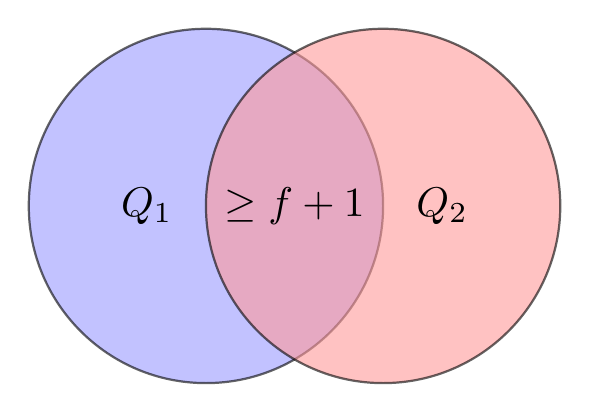
\begin{tikzpicture}[scale=1.5, every node/.style={transform shape}]
    \draw[fill=blue!40, opacity=0.6, draw=black, thick] (0,0) circle (1.5);
    \draw[fill=red!40, opacity=0.6, draw=black, thick] (1.5,0) circle (1.5);
    \node[text=black, font=\bfseries] at (-0.5,0) {$Q_1$};
    \node[text=black, font=\bfseries] at (2.0,0) {$Q_2$};
    \node[text=black, font=\bfseries] at (0.75,0) {$\ge f+1$};
\end{tikzpicture}
\caption{Quorum Intersection in pBFT}
\end{figure}
\section{The Protocol in the Normal Case}

\subsection{State Machine Replication}
pBFT models the service as a deterministic state machine. All replicas must start in the same initial state and execute operations identically. The primary challenge is to guarantee that all honest replicas execute the same requests in the exact same total order. The system progresses through sequences of \textbf{views}. In each view, one replica assumes the role of the \textbf{primary (leader)}, while the remaining replicas act as \textbf{backups}.

\subsection{The 3-Phase Protocol}
To tolerate Byzantine faults, the protocol requires three phases of communication:

\begin{enumerate}
    \item \textbf{Pre-prepare:} The primary receives a client request, assigns a sequence number to it, and broadcasts a \texttt{PRE-PREPARE} message to the backups.
    \item \textbf{Prepare:} A backup verifies the message and broadcasts a \texttt{PREPARE} message to all other replicas. A node considers itself ``prepared'' once it has collected the original request/message plus a quorum of $2f$ matching \texttt{PREPARE} messages.
    \item \textbf{Commit:} Upon becoming ``prepared,'' the node broadcasts a \texttt{COMMIT} message. When a node aggregates $2f+1$ matching \texttt{COMMIT} messages, it achieves local commit status, executes the operation, and returns the response to the client.
\end{enumerate}

\begin{figure}[H]
\centering
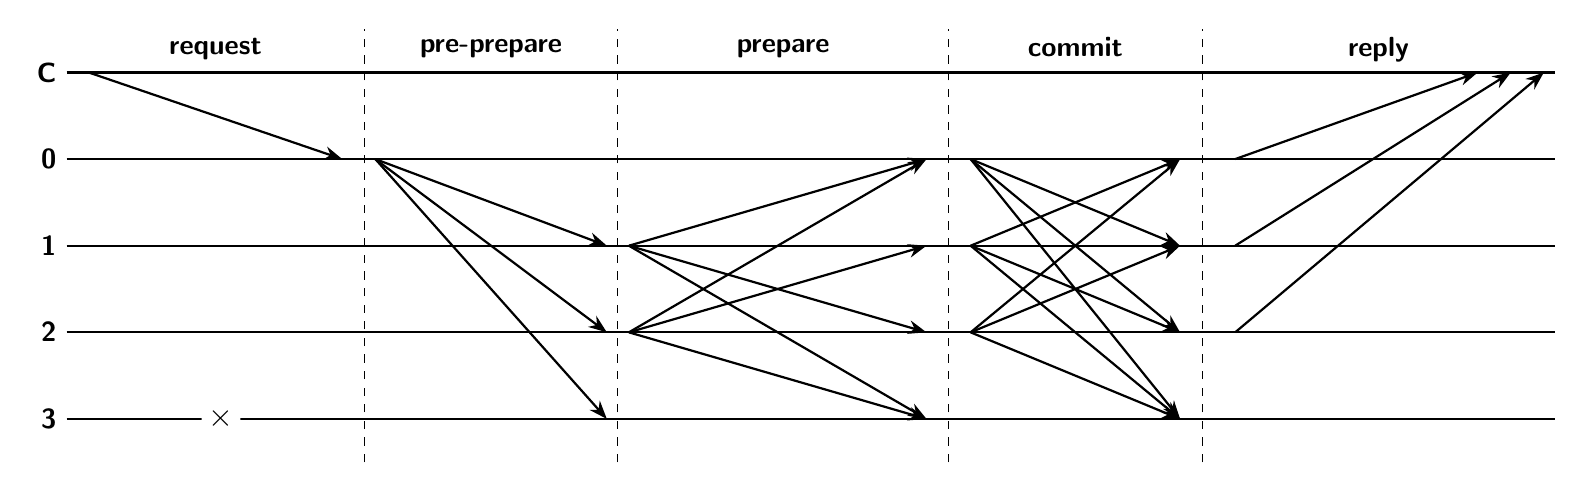
\begin{tikzpicture}[
    xscale=1.4, 
    yscale=1.1, 
    >=Stealth, 
    thick,
    % Definición de estilo para las etiquetas de las fases
    phase label/.style={font=\sffamily\bfseries, text depth=0pt}
]
    % --- 1. LÍNEAS HORIZONTALES (LÍNEAS DE VIDA) ---
    % Alturas fijas para C, 0, 1, 2, 3 (invertido para que C quede arriba)
    \draw (0,4) node[left, font=\sffamily\bfseries] {C} -- (13.5,4);
    \draw (0,3) node[left, font=\sffamily\bfseries] {0} -- (13.5,3);
    \draw (0,2) node[left, font=\sffamily\bfseries] {1} -- (13.5,2);
    \draw (0,1) node[left, font=\sffamily\bfseries] {2} -- (13.5,1);
    \draw (0,0) node[left, font=\sffamily\bfseries] {3} -- (13.5,0);

    % --- 2. LÍNEAS VERTICALES DISCONTINUAS (FASES) ---
    \draw[dashed, thin] (2.7, -0.5) -- (2.7, 4.5);
    \draw[dashed, thin] (5.0, -0.5) -- (5.0, 4.5);
    \draw[dashed, thin] (8.0, -0.5) -- (8.0, 4.5);
    \draw[dashed, thin] (10.3, -0.5) -- (10.3, 4.5);

    % --- 3. ETIQUETAS DE LAS FASES ---
    \node[phase label] at (1.35, 4.3) {request};
    \node[phase label] at (3.85, 4.3) {pre-prepare};
    \node[phase label] at (6.50, 4.3) {prepare};
    \node[phase label] at (9.15, 4.3) {commit};
    \node[phase label] at (11.90, 4.3) {reply};

    % --- 4. MARCA DE FALLO (X en el Nodo 3) ---
    \node[font=\sffamily\bfseries\Large, text=black, fill=white, inner sep=1pt, circle, scale=0.8] at (1.4, 0) {$\mathbf{\times}$};

    % --- 5. SOLICITUD (REQUEST) ---
    \draw[->] (0.2,4) -- (2.5,3);

    % --- 6. FASE PRE-PREPARE ---
    % Desde el Nodo 0 (líder) hacia los respaldos (1, 2, 3) al final de la fase
    \draw[->] (2.8,3) -- (4.9,2);
    \draw[->] (2.8,3) -- (4.9,1);
    \draw[->] (2.8,3) -- (4.9,0);

    % --- 7. FASE PREPARE ---
    % Intercambio cruzado total entre nodos 1 y 2, y emisión hacia 0 y 3
    % Mensajes desde Nodo 1:
    \draw[->] (5.1,2) -- (7.8,3);
    \draw[->] (5.1,2) -- (7.8,1);
    \draw[->] (5.1,2) -- (7.8,0);

    % Mensajes desde Nodo 2:
    \draw[->] (5.1,1) -- (7.8,3);
    \draw[->] (5.1,1) -- (7.8,2);
    \draw[->] (5.1,1) -- (7.8,0);

    % --- 8. FASE COMMIT ---
    % Intercambio generalizado todos a todos (Nodos activos: 0, 1, 2 hacia 0, 1, 2, 3)
    % Mensajes desde Nodo 0:
    \draw[->] (8.2,3) -- (10.1,2);
    \draw[->] (8.2,3) -- (10.1,1);
    \draw[->] (8.2,3) -- (10.1,0);

    % Mensajes desde Nodo 1:
    \draw[->] (8.2,2) -- (10.1,3);
    \draw[->] (8.2,2) -- (10.1,1);
    \draw[->] (8.2,2) -- (10.1,0);

    % Mensajes desde Nodo 2:
    \draw[->] (8.2,1) -- (10.1,3);
    \draw[->] (8.2,1) -- (10.1,2);
    \draw[->] (8.2,1) -- (10.1,0);

    % --- 9. FASE DE RESPUESTA (REPLY) ---
    % Respuestas consecutivas de los nodos honestos (0, 1, 2) hacia el cliente C
    \draw[->] (10.6,3) -- (12.8,4);
    \draw[->] (10.6,2) -- (13.1,4);
    \draw[->] (10.6,1) -- (13.4,4);

\end{tikzpicture}
\caption{Sequence diagram of the normal case operation where node 3 is faulty}
\end{figure}
\section{Garbage Collection and Checkpoints}
In pBFT, each replica must store messages in a log. However, memory resources necessitate a garbage collection mechanism to periodically truncate this log so that it does not grow indefinitely.

\subsection{Stable Checkpoint Generation}
The protocol periodically generates cryptographic proofs (e.g., every 100 requests) confirming that a consolidated state is correct, which is referred to as a \textbf{checkpoint}. When a replica generates a checkpoint, it broadcasts a \texttt{CHECKPOINT} message to all other replicas.

This checkpoint transitions into a \textbf{stable checkpoint} once the replica successfully aggregates a total of $2f+1$ identical checkpoint messages from other nodes. This quorum proves that an honest majority of the system agrees on the current state. Upon achieving stability, the replica safely purges all messages related to the \texttt{pre-prepare}, \texttt{prepare}, and \texttt{commit} phases that have sequence numbers equal to or lower than that of the stable checkpoint.

\subsection{Watermarks and State Transfer}
The protocol establishes strict operating boundaries defined by two watermarks: the low watermark ($h$), which matches the sequence number of the latest stable checkpoint, and the high watermark ($H = h + k$). This range restricts the sequence numbers of valid operations, preventing a malicious leader from intentionally assigning massive sequence numbers to exhaust memory space. Furthermore, pBFT utilizes a hierarchical state tree combined with a \textit{copy-on-write} memory management technique to perform efficient state transfers and mathematical updates without halting the entire system, thereby accelerating the recovery of slow or lagging nodes.
\section{View Changes (Leader Fault Tolerance)}
To maintain the system's liveness when the primary node fails or acts maliciously, nodes transition through a succession of configurations called \textit{views}.

Backup nodes monitor the primary's behavior using timers (\textit{timeouts}). A backup initiates a timer upon receiving a request; if the timer expires without any progress in processing, the backup assumes the leader is defective and halts the execution of the normal protocol.

The node ceases to accept normal operation messages and broadcasts a \texttt{VIEW-CHANGE} message requesting a transition to the next view ($v+1$). To be valid, this message appends cryptographic proofs of its latest stable checkpoint as well as all operations that had already reached the locally prepared state.

The new leader, designated by the formula $v \bmod N$ (where $N$ is the total number of nodes), takes control after aggregating at least $2f$ of these messages. It then issues a \texttt{NEW-VIEW} message containing consolidated proofs to resume the interrupted operations, ensuring that no operation already confirmed to a client is ever lost, and using null operations (\textit{no-ops}) to fill any empty slots in the sequence numbers. 

To prevent abuses, the protocol implements forced rotation and exponential timeout backing off in case of repetitive, failed view changes.
\section{Cryptography, Practical Optimizations, and Performance}
pBFT resolves cryptographic latency bottlenecks by reserving expensive public-key signatures (such as RSA) exclusively for critical operational transitions like view changes. In the normal case, it employs symmetric-key cryptography \textbf{Message Authentication Codes (MACs)} for the overwhelming majority of interactions, which perform orders of magnitude faster.

Additionally, it optimizes data transmission overhead by instructing only one designated replica to send the complete response payload back to the client, while the remaining nodes transmit only small cryptographic digests. For high-demand environments, pBFT utilizes request batching within a single consensus sequence and enables a fast path for read-only operations.

\subsection{Byzantine File System (BFS) Architecture}
To empirically demonstrate the "practical" value of pBFT, the authors developed a replication library upon which they implemented the Byzantine-Fault-tolerant File System (BFS). This filesystem supports the standard NFS V2 network protocol transparently, requiring no modifications to either the client or the original kernel server.

\begin{figure}[h!]
\centering
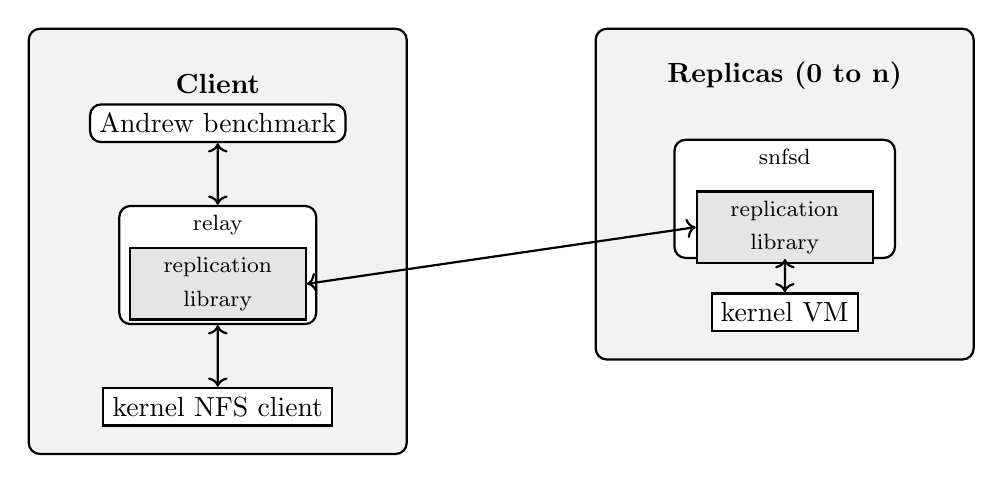
\begin{tikzpicture}[xscale=1.2, yscale=1.2, thick]
    % Client
    \draw[rounded corners, fill=black!5] (0,0) rectangle (4,4.5) node[pos=0.5, yshift=2.0cm] {\textbf{Client}};
    \node[draw, rounded corners, fill=white] (andrew) at (2, 3.5) {Andrew benchmark};
    
    \node[draw, rounded corners, minimum width=2.5cm, minimum height=1.5cm, fill=white] (relay_box) at (2, 2) {};
    \node[anchor=north] at (relay_box.north) {\footnotesize relay};
    \node[draw, fill=gray!20, text width=2cm, align=center] (replib_c) at (2, 1.8) {\footnotesize replication\\ \footnotesize library};
    
    \node[draw, fill=white] (knfs) at (2, 0.5) {kernel NFS client};
    
    \draw[<->] (andrew) -- (relay_box);
    \draw[<->] (relay_box) -- (knfs);

    % Replica
    \draw[rounded corners, fill=black!5] (6,1) rectangle (10,4.5) node[pos=0.5, yshift=1.5cm] {\textbf{Replicas (0 to n)}};
    
    \node[draw, rounded corners, minimum width=2.8cm, minimum height=1.5cm, fill=white] (daemon0) at (8, 2.7) {};
    \node[anchor=north] at (daemon0.north) {\footnotesize snfsd};
    \node[draw, fill=gray!20, text width=2cm, align=center] (replib_0) at (8, 2.4) {\footnotesize replication\\ \footnotesize library};
    
    \node[draw, fill=white] (kvm) at (8, 1.5) {kernel VM};
    
    \draw[<->] (daemon0) -- (kvm);

    % Connections
    \draw[<->] (replib_c.east) -- (replib_0.west);
\end{tikzpicture}
\caption{Simplified BFS Architecture}
\end{figure}

\begin{figure}[H]
\centering
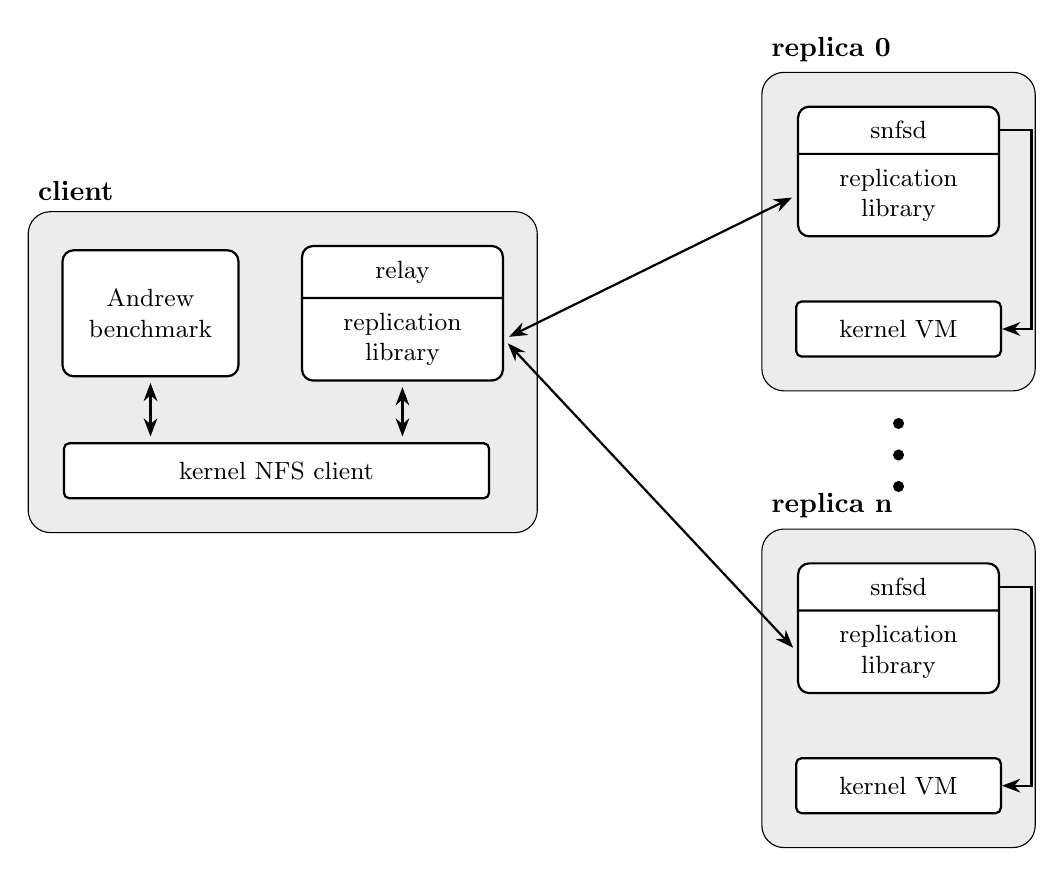
\begin{tikzpicture}[
    >=Stealth,
    thick,
    % Estilo para las cajas divididas (relay y snfsd)
    splitbox/.style={
        rectangle split, 
        rectangle split parts=2, 
        draw, 
        rounded corners=4pt, 
        fill=white,
        text width=2.2cm, 
        align=center, 
        font=\small,
        inner sep=5pt
    },
    % Estilo para las cajas simples (Andrew benchmark)
    innerbox/.style={
        draw, 
        rounded corners=4pt, 
        fill=white, 
        minimum width=2.2cm, 
        minimum height=1.6cm, 
        text width=2cm, 
        align=center, 
        font=\small
    },
    % Estilo para el Kernel
    kernelbox/.style={
        draw, 
        rounded corners=2pt,
        fill=white, 
        minimum height=0.7cm, 
        align=center, 
        font=\small
    },
    % Estilo para las cajas exteriores (Sombreado Gris)
    outerbox/.style={
        draw, 
        rounded corners=8pt, 
        fill=gray!15, % <-- Sombreado gris añadido
        inner sep=12pt
    }
]

    % ==========================================
    % CLIENTE (BLOQUE IZQUIERDO)
    % ==========================================
    % Componentes internos
    \node[innerbox] (andrew) at (0, 0) {Andrew\\benchmark};
    \node[splitbox] (relay) at (3.2, 0) {relay\nodepart{two}replication\\library};
    \node[kernelbox, minimum width=5.4cm] (knfs) at (1.6, -2.0) {kernel NFS client};
    
    % Flechas internas del cliente
    \draw[<->, shorten >=2pt, shorten <=2pt] (andrew.south) -- (andrew.south |- knfs.north);
    \draw[<->, shorten >=2pt, shorten <=2pt] (relay.south) -- (relay.south |- knfs.north);
    
    % Caja exterior ajustada al contenido
    \begin{scope}[on background layer]
        \node[outerbox, fit=(andrew) (relay) (knfs)] (clientbox) {};
    \end{scope}
    \node[anchor=south west, font=\bfseries] at (clientbox.north west) {client};


    % ==========================================
    % RÉPLICA 0 (BLOQUE SUPERIOR DERECHO)
    % ==========================================
    % Componentes internos
    \node[splitbox] (snfsd0) at (9.5, 1.8) {snfsd\nodepart{two}replication\\library};
    \node[kernelbox, minimum width=2.6cm] (kvm0) at (9.5, -0.2) {kernel VM};
    
    % Flecha interna de la réplica (sale de snfsd, baja y entra a la VM)
    \draw[->] (snfsd0.text east) -- ++(0.4,0) |- (kvm0.east);
    
    % Caja exterior ajustada
    \begin{scope}[on background layer]
        \node[outerbox, fit=(snfsd0) (kvm0)] (rep0box) {};
    \end{scope}
    \node[anchor=south west, font=\bfseries] at (rep0box.north west) {replica 0};


    % ==========================================
    % PUNTOS SUSPENSIVOS VERTICALES
    % ==========================================
    \fill (9.5, -1.4) circle (2pt);
    \fill (9.5, -1.8) circle (2pt);
    \fill (9.5, -2.2) circle (2pt);


    % ==========================================
    % RÉPLICA N (BLOQUE INFERIOR DERECHO)
    % ==========================================
    % Componentes internos
    \node[splitbox] (snfsdn) at (9.5, -4.0) {snfsd\nodepart{two}replication\\library};
    \node[kernelbox, minimum width=2.6cm] (kvmn) at (9.5, -6.0) {kernel VM};
    
    % Flecha interna de la réplica (sale de snfsd, baja y entra a la VM)
    \draw[->] (snfsdn.text east) -- ++(0.4,0) |- (kvmn.east);
    
    % Caja exterior ajustada
    \begin{scope}[on background layer]
        \node[outerbox, fit=(snfsdn) (kvmn)] (repnbox) {};
    \end{scope}
    \node[anchor=south west, font=\bfseries] at (repnbox.north west) {replica n};


    % ==========================================
    % CONEXIONES DE RED
    % ==========================================
    % Conectan la librería de replicación del cliente (parte 2 del relay) 
    % con las librerías de replicación de las réplicas (parte 2 del snfsd)
    \draw[<->, shorten >=2pt, shorten <=2pt] (relay.two east) -- (snfsd0.two west);
    \draw[<->, shorten >=2pt, shorten <=2pt] (relay.two east) -- (snfsdn.two west);

\end{tikzpicture}
\caption{BFS Architecture Diagram}
\end{figure}

By subjecting BFS to the demanding \textit{Andrew benchmark}, the authors proved that the performance penalty incurred is remarkably small:

\begin{table}[h!]
\centering
\begin{tabular}{|l|c|c|c|}
\hline
\textbf{Benchmark Phases} & \textbf{BFS (pBFT)} & \textbf{BFS-nr (Unrep.)} & \textbf{NFS-std (Commercial)} \\ \hline
1. Create directories & 0.55 & 0.35 & 1.75 \\ \hline
2. Copy files & 9.24 & 5.08 & 9.46 \\ \hline
3. Read metadata & 7.24 & 6.11 & 5.36 \\ \hline
4. Read data & 8.77 & 7.41 & 6.60 \\ \hline
5. Compile and link & 38.68 & 32.12 & 39.35 \\ \hline
\textbf{Total Time (seconds)} & \textbf{64.48} & \textbf{51.07} & \textbf{62.52} \\ \hline
\end{tabular}
\caption{Andrew Benchmark Results. The pBFT (BFS) execution time proved to be only roughly 3\% slower than or even competitive with industry-standard commercial NFS.}
\end{table}
\section{Advanced Concepts and Contemporary Use Cases}
The base pBFT algorithm assumes that no more than $f$ failures occur during the entire lifespan of the system. However, computing systems operate for months or years, increasing the statistical probability of exceeding this cumulative limit of $f$ failures. To bridge this gap, the system employs a technique called \textbf{Proactive Recovery}. 

Instead of waiting for failures to be detected, nodes cycle through reboots and recoveries proactively (e.g., every 10–20 minutes) utilizing a secure hardware coprocessor, which stores the original source code in read-only memory (ROM). During this recovery process, new secret keys are generated to prevent identity theft. This drastically transforms the model: rather than tolerating $f$ failures over its entire lifespan, pBFT tolerates $f$ \textit{simultaneous} failures within a small, defined window of time.

\subsection{The pBFT Renaissance}
Initially rejected by the industry in favor of prevention models and firewalls, pBFT was long viewed as a purely academic problem. However, it has experienced an explosive renaissance driven by the \textbf{Zero Trust} cybersecurity paradigm (assuming the network is already breached) and the innovations brought by the blockchain era.

Unlike the invention of \textbf{Bitcoin}, whose Proof-of-Work consensus tolerates malicious participants but heavily penalizes performance (high latency, massive energy consumption, and lack of strict linearizability or immediate finality due to potential \textit{forks}), pBFT offers immediate, absolute finality and high throughput in closed groups. Today, pBFT and its derivatives serve as the architectural standard in financial systems and enterprise \textit{Hyperledgers} such as \textbf{Stellar} and \textbf{IBM Hyperledger}, solving corporate consensus challenges at commercial speeds.
\section{Conclusions}

Practical Byzantine Fault Tolerance (pBFT) successfully bridged the gap between theoretical models of Byzantine fault tolerance and real-world distributed systems. By optimizing cryptographic operations---relying primarily on efficient symmetric Message Authentication Codes (MACs) and reserving expensive public-key cryptography only for critical view-change procedures---pBFT demonstrated that resilience against arbitrary, malicious node behavior could be achieved without crippling system performance. The empirical results from the Byzantine-Fault-tolerant File System (BFS) proved that pBFT incurs merely a marginal overhead compared to standard, unreplicated systems.

Furthermore, mechanisms such as garbage collection via stable checkpoints and proactive recovery through secure hardware coprocessors address the limitations of unbounded log growth and long-term security, ensuring the protocol remains robust over extended lifespans. 

While initially considered an academic exercise due to the industry's reliance on perimeter-based security, the rise of the Zero Trust security paradigm and decentralized networks has catalyzed a renaissance for pBFT. Its ability to provide immediate transaction finality, strict linearizability, and high throughput without the massive energy consumption associated with Proof-of-Work mechanisms has established it as the foundational consensus architecture for modern permissioned blockchains, such as Hyperledger, and federated financial networks. Ultimately, pBFT remains a seminal work, proving that achieving high-performance consensus in untrusted environments is both mathematically rigorous and practically viable.

\end{document}